% !TEX TS-program = xelatex

% Inicializace tulthesis
\documentclass[FM,Proj]{tulthesis}
\usepackage{polyglossia}
\setdefaultlanguage{czech}
\usepackage{xevlna}

% Pro umisťování obrázků
%\usepackage{float}

% Pro seznam použité literatury
\usepackage[backend=biber, style=iso-numeric]{biblatex}
\addbibresource{zdroje.bib}

% Titulní strana
\TULtitle{Vývoj akční videohry zasazené do prostředí FM}{Development of an action video game set in FM}
\TULprogramme{B0613A140005}{Informační technologie}{Information technology}
%\TULbranch{B0613A140005AI}{Aplikovaná informatika}{Applied Informatics}
\TULauthor{Radek Mocek}
\TULsupervisor{Ing. Jan Hybš}
\TULyear{2023}

\begin{document}
	% Prohlášení
	\ThesisStart{male}
	
	% Abstrakt česky
	\begin{abstractCZ}
		Český abstrakt
	\end{abstractCZ}
	
	% Klíčová slova česky
	\begin{keywordsCZ}
		klíčová slova česky
	\end{keywordsCZ}
	\vspace{2cm}
	
	% Abstrakt anglicky
	\begin{abstractEN}
		English abstract
	\end{abstractEN}
	
	% Klíčová slova anglicky
	\begin{keywordsEN}
		keywords in English
	\end{keywordsEN}
	
	% Obsah
	\tableofcontents
	
	% Seznam obrázků
	\listoffigures
	
	% Seznam tabulek
	%\listoftables
	
	\clearpage
	
	% Zkratky
%	\begin{abbrList}
%		\textbf{TUL} & Technická univerzita v~Liberci \\
%		\textbf{FM} & Fakulta mechatroniky, informatiky a mezioborových studií Technické univerzity v~Liberci
%	\end{abbrList}
	
	% Začátek hlavního textu
	\chapter{Úvod}
	
	\chapter{Herní engine Unity}
	% Zjistěte, jaké nástroje a knihovny jsou dostupné pro vývoj 2D videoher v Unity enginu. Prozkoumejte jejich funkce, výhody a nevýhody a jak se dají použít pro vaše potřeby.
	% * [X] Unity obecně
	% * [X] Představení editoru a základních prvků (gameObject, prefab, scéna, asset)
	% * [X] Sprite, animace, 9slicing
	% * [X] Tilemap – https://unity.com/how-to/optimize-performance-2d-games-unity-tilemap
	% * [ ] SpriteShape – https://docs.unity3d.com/Packages/com.unity.2d.spriteshape@7.0/manual/index.html
	% * [ ] URP, především 2DLight
	% * [ ] Balíčky – CineMachine, VectorGraphics, InputSystem, ...; asset store
	% * [ ] Canvas
	
	% Statistika užití jednotlivých enginů – https://itch.io/game-development/engines/most-projects
	
	%free, (verze?), mono vs il2cpp, podporované platformy
	Unity je multiplatformní herní engine s uzavřeným kódem vyvíjený společností Unity Technologies. První veřejná verze vyšla v roce 2005 a od té doby si Unity vybudovalo početnou komunitu a stalo se populární především mezi nezávislými vývojáři. Unity poskytuje nástroje pro vývoj 2D a 3D her, využívá se ale také ve filmovém nebo automobilovém průmyslu. Základní verze Unity je zdarma.
	
	\section{Editor a základní stavební prvky}
	
	Základem každého Unity projektu jsou tzv. assety. Asset je jakýkoliv prvek, který je v projektu využit k vytvoření finální hry nebo aplikace. Asset je reprezentován ve formě souboru a často se jedná o prvek tvořící audiovizuální stránku hry (např. 3D model, textura, sprite, zvukový soubor). Dalšími důležitými assety jsou scény, které slouží jako herní prostředí a uchovávají v sobě ostatní assety v podobě herních objektů, a skripty psané v jazyce C\#, které definují chování daných herních objektů.  \cite{UnityDocsAssetWorkflow}
	
	Každý prvek použitý ve scéně je herním objektem. Herní objekt nemá sám o sobě žádnou funkcionalitu, jedná se pouze o kontejner pro komponenty, které pak určují jeho vzhled a chování \cite{UnityDocsGameObject}. Základní komponenta umístěná na téměř každém herním objektu je \textit{Transform}, která určuje jeho umístění, rotaci a měřítko v prostoru scény. Do některých komponent lze jako argument dosadit asset, např. dosazení spritu do komponenty \textit{Sprite Renderer}, která zajistí jeho vykreslení. Pro opakované použití stejného herního objektu je vhodné z něj vytvořit tzv. prefab. Prefab je asset reprezentující herní objekt a změna hodnot v jeho komponentách se projeví ve všech jeho instancích.
	
	Unity editor lze ve svém výchozím rozložení rozdělit na čtyři základní části. Dole se nachází průzkumník projektu, ten umožňuje procházení, třídění a importování assetů do projektu. Uprostřed je editor scény, ve kterém si lze scénu prohlížet a vybírat v ní obsažené herní objekty pro následné úpravy. Nalevo od editoru scény je průzkumník její hierarchie, v něm jsou vidět všechny herní objekty (včetně instancí prefabů), které jsou obsaženy v právě prohlížené scéně. V neposlední řadě se na pravé straně nachází inspektor, který zobrazuje detailní informace o právě vybraném herním objektu nebo assetu a umožňuje jeho modifikaci. Pro herní objekt zobrazuje všechny jeho komponenty, zatímco u assetů se zobrazení informací liší podle typu zvoleného assetu.
	
	\begin{figure}[ht]
		\centering
		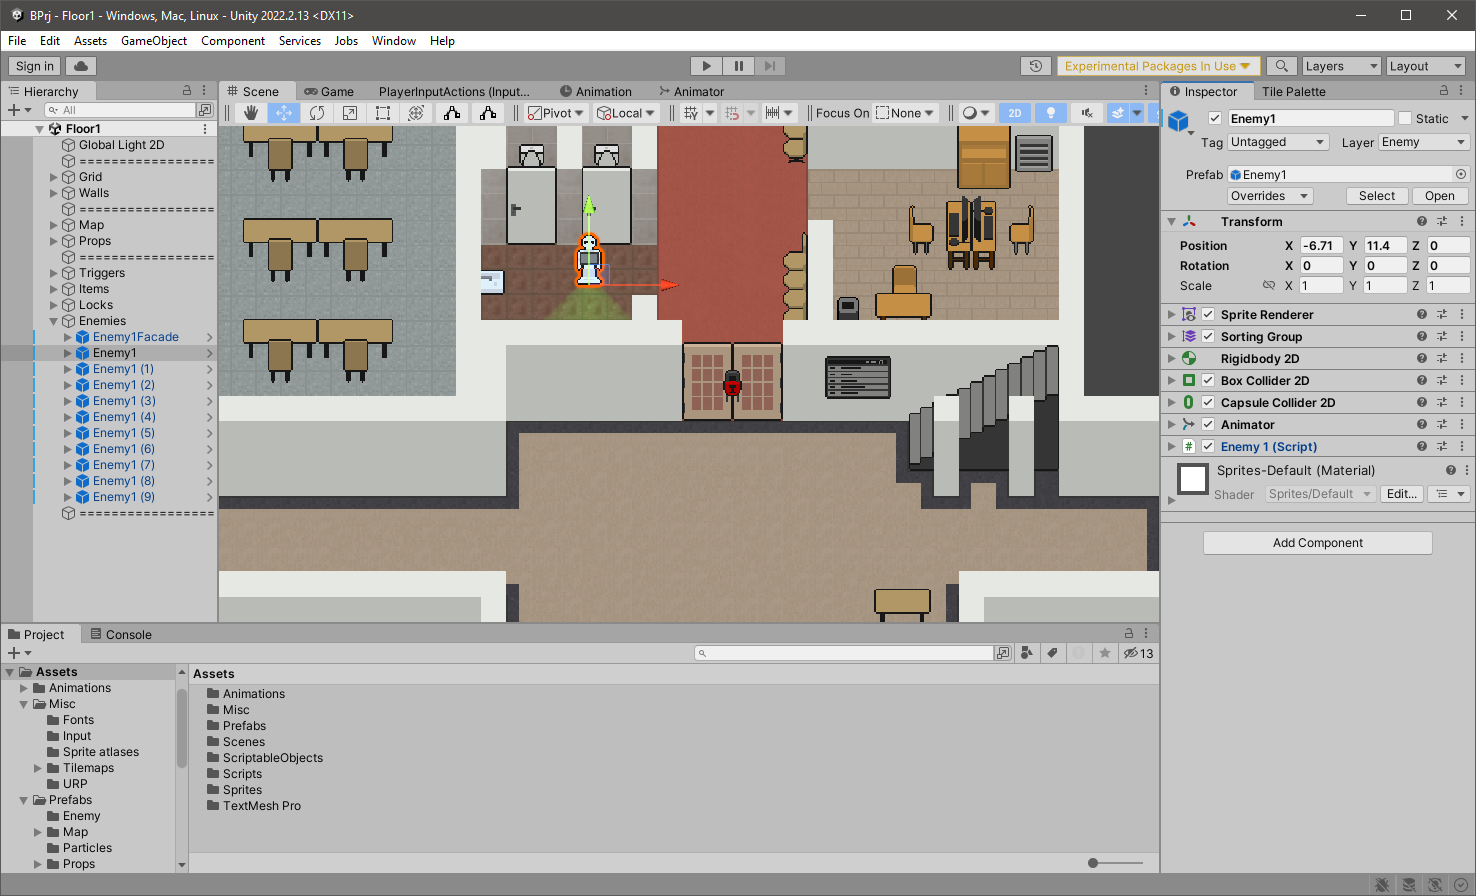
\includegraphics[width=\textwidth]{img/UnityEditor}
		\caption{Unity editor}
	\end{figure}
	
	\section{2D tvorba}
	
	Unity vzniklo původně jako engine pro vývoj 3D her a nástroje pro 2D tvorbu byly přidány až v pozdějších verzích. Volba mezi 2D a 3D je prvním krokem při zakládání nového projektu, rozdíl mezi nimi ale není velký a oba přístupy lze během vývoje kombinovat. Hlavním viditelným rozdílem pro 2D projekty je editor scény, který je přepnut do dvourozměrného režimu. V tomto módu je změněn význam osy Z, která místo popisu třetího rozměru značí hloubku (podobně jako např. vlastnost z-index v CSS). \cite{Unity2DAnnouncement}
	
	\subsection{Sprite} %spriteshape, atlas;
	
	Sprite je jeden z nejběžnějších assetů ve 2D videohře. V Unity vzniká přetažením bitmapového obrázku do průzkumníka projektu (obvykle do složky \textit{Sprites}) a má několik vlastností, které lze změnit v inspektoru. Za zmínku stojí hodnota \textit{Pixels Per Unit}, která určuje, kolik pixelů ve spritu odpovídá jednotce vzdálenosti v herním světě (ve scéně). Druhý důležitý parametr je \textit{Pivot}, ten značí bod, kolem kterého sprite rotuje, a také může ovlivnit pořadí vykreslení daného spritu.
	
	Každý sprite nemusí být reprezentován samostatným bitmapovým souborem, místo toho lze naimportovat tzv. spritesheet. Jedná se o větší obrázek obsahující více spritů uspořádaných do mřížky, ty jsou pak rozděleny na jednotlivé assety v nástroji editor spritů. Tento nástroj také umožňuje připravit obrázek pro specifický typ škálování zvaný 9-slicing (obrázek \ref{img9Slicing}).
	
	\begin{figure}[ht]
		\centering
		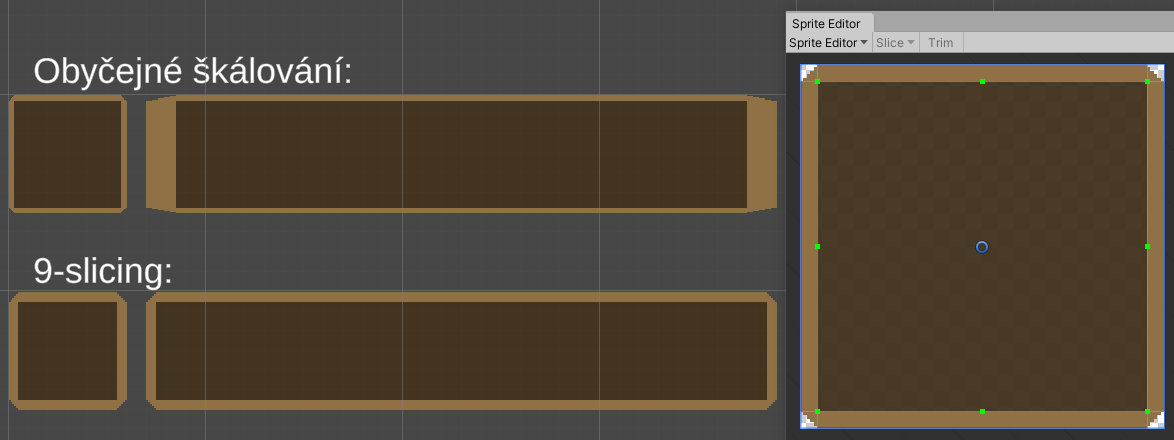
\includegraphics[width=\textwidth]{img/9Slicing}
		\caption{9-slicing}
		\label{img9Slicing}
	\end{figure}
	
	\subsection{Animace}
	
	Unity umožňuje tvorbu animací po jednotlivých snímcích, kdy je každý snímek animace reprezentován samostatným spritem. Jednotlivé sprity jsou pokládány na časovou osu v nástroji \textit{Animation}. Nevýhoda této metody se projeví v situaci, kdy je potřeba např. nějaké postavě změnit barvu vlasů. V tomto případě je nutné všechny sprity všech animací postavy upravit v (externím) grafickém editoru. Problém by šel také vyřešit tvorbou speciálního shaderu nebo editací jednotlivých pixelů ze skriptu, nejedná se ale o standardní postupy. Alternativně lze použít metodu trojúhelníkové sítě a kostry. Jedná se o běžný způsob tvorby 3D animací, Unity jej ale umožňuje aplikovat i na 2D sprity.
	
	Každý herní objekt schopný animace musí mít přiřazený asset typu \textit{Animator Controller} (dále jen AC). Ten je vytvořen a upravován přímo v Unity editoru a jeho diagram připomíná schéma stavového automatu. Všechny animace, ve kterých se herní objekt může nacházet, jsou v diagramu reprezentovány obdélníkem. Obdélníky lze spojovat šipkami, které značí podmíněný přechod mezi jednotlivými animacemi. AC umožňuje definovat si v něm interní proměnné (\textit{parameters}), jejichž hodnoty lze měnit ze skriptu a využívají se pro sestavení podmínek přechodu. AC diagramy složitějších herních objektů mohou značně nabýt na složitosti, je možné se jim ale vyhnout. Volání funkce \textit{Animator.CrossFade} dovoluje změnit animaci kdykoliv bez ohledu na stav AC diagramu.
	
	\subsection{Tilemap}
	
	Tilemap je nástroj pro tvorbu herních světů převážně ve 2D. Základem je pravidelná mřížka, do které jsou vkládány dlaždice (\textit{tiles}). Dlaždice je malý sprite nakreslený tak, aby více dlaždic položených vedle sebe vypadalo přirozeně a dala se z nich takto poskládat celá herní mapa. Využitím tilemap lze tvořit velké herní mapy bez dopadu na výkon a zároveň je kdykoliv snadno editovat. Unity nabízí obdélníkovou tilemap (nejběžnější, vhodné pro plošinovky a top-down videohry), ale také šestiúhelníkovou nebo izometrickou. V jedné scéně se může nacházet více tilemap a každá může být v jiné vrstvě. To např. umožňuje, aby se některé dlaždice vykreslovaly před a některé za postavou hráče.
	
	\textit{Rule Tile} je speciální druh dlaždice, která mění svůj vzhled na základě jednoduchých nastavitelných pravidel. Sprite této dlaždice se mění podle toho, zdali se v jejím okolí nachází dlaždice stejného druhu. Funkcionalita je ale omezená, nelze např. nastavit, aby dlaždice reagovala na své sousedy z jiných vrstev nebo na jiné dlaždice ve stejné vrstvě.
	
	\begin{figure}[ht]
		\centering
		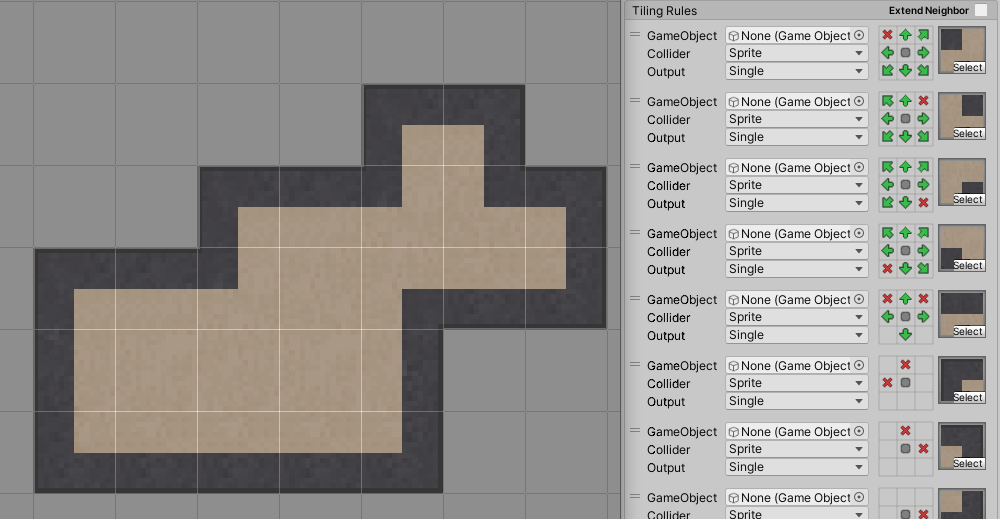
\includegraphics[width=\textwidth]{img/RuleTile}
		\caption{Rule Tile}
	\end{figure}
	
	\subsection{Universal Render Pipeline}

	Universal Render Pipeline (URP) je skriptovatelný vykreslovací řetězec, který je do Unity projektu přidán ve formě balíku. Otázka použití alternativního vykreslovacího řetězce bývá častější u vývoje 3D her, i pro 2D projekty ale URP přináší nové grafické možnosti. Tím nejzásadnějším jsou dvě nové komponenty \textit{Light 2D} a \textit{Shadow Caster 2D}, díky kterým lze do scény přidat dynamická světla a stíny.
	
	\chapter{Návrh videohry}
	% Vymyslete koncept a herní mechaniky pro 2D top-down videohru.	Rozmyslete si, jak bude hráč ovládat postavu, jaké budou cíle a výzvy ve hře a jaké prostředí a překážky budou hráči čelit.
	
	\chapter{Návrh umělé inteligence}
	% Vytvořte jednoduchý systém umělé inteligence pro nepřátelské jednotky ve hře, který bude řízen stavovým automatem. Uvažujte o různých stavech, ve kterých se může nepřítel nacházet (např. hlídka, útok, ústup), a jak tyto stavy ovlivní chování nepřátelských jednotek.
	
	\chapter{Implementace}
	% Implementace demonstrativní videohry v prostředí budovy FM TUL.
	
	\chapter{Kritické zhodnocení}
	% Výslednou videohru kriticky zhodnoťte a navrhněte případné rozšíření či vylepšení.
	
	\chapter{Závěr}
	
	% Zdroje
	\chapter*{Seznam použité literatury}
	\addcontentsline{toc}{chapter}{Seznam použité literatury}
	\printbibliography[heading=none]
	
\end{document}